\documentclass[conference]{IEEEtran}
\IEEEoverridecommandlockouts
\usepackage[T1]{fontenc}
\usepackage[utf8]{inputenc}
\usepackage{amsmath,amssymb,amsfonts}
\usepackage{graphicx}
\usepackage{textcomp}
\usepackage{booktabs}
\usepackage{array}
\usepackage{url}
\usepackage{tikz}
\usetikzlibrary{positioning,shapes.geometric,arrows.meta}
\usepackage{newunicodechar}
\newunicodechar{−}{\ensuremath{-}}
\newunicodechar{→}{\ensuremath{\rightarrow}}
\newunicodechar{←}{\ensuremath{\leftarrow}}
\newunicodechar{≈}{\ensuremath{\approx}}
\newunicodechar{≤}{\ensuremath{\leq}}
\newunicodechar{≥}{\ensuremath{\geq}}
\newunicodechar{×}{\ensuremath{\times}}
\newunicodechar{±}{\ensuremath{\pm}}
\newunicodechar{·}{\ensuremath{\cdot}}
\newunicodechar{∈}{\ensuremath{\in}}
\newunicodechar{÷}{\ensuremath{\div}}
\newunicodechar{⋈}{\ensuremath{\bowtie}}

% Harvard-style reference list (QMUL MSc guide §8.2) inside the IEEE layout
\newcommand{\refentry}{\par\noindent\hangindent=1.2em\hangafter=1}
\usepackage{algorithm}
\usepackage{algpseudocode}

\begin{document}

\title{Prompt Cost Optimisation for Speculative Parallelism in Text-to-SQL:
Schema Pruning, a Semantic Fact Store, and Cache-Stable Structure}

\author{\IEEEauthorblockN{Pasha Gorenkin}
\IEEEauthorblockA{\textit{School of Electronic Engineering and Computer Science} \\
\textit{Queen Mary University of London}\\
London, United Kingdom \\
gorenkinp@gmail.com}
}

\maketitle

\begin{abstract}
Large language models deployed as tool-using SQL agents buy reliability with
\emph{speculative parallelism}: $N$ replicas attempt one task and a coordinator
selects an answer. The resulting waste is usually sought in their duplicated
queries. It is larger in the prompt. Because chat APIs are stateless, billed
input per task is approximately $N \times T \times \mathrm{price}(P + \bar{H})$,
or replicas times turns times the price of a static prefix plus an accumulated
history, so a schema is re-billed some sixty times for a six-turn, ten-replica
task. That identity has three factors, and this paper
evaluates one method against each: recall-aware schema pruning, a semantic fact
store, and cache-stable prompt structure, measured in isolation and composed,
on BIRD across three API models, on a 50-task subset and over all 500 tasks.

Repricing is the unconditional win: cache-stable structure changes no content
byte, leaves raw consumption unmoved in fourteen of fifteen configurations, and
removes 18.8--86.0\% of billed input in all fifteen. Raw and billed tokens are
separate ledgers, moving in opposite directions in one configuration with both
intervals excluding zero. Prefix reduction is conditional on recall, and
the condition is measurable offline: pruning removes 9.9--19.7\% of tokens where
every gold table survives and \emph{adds} 32--156\% where one does not, leaving
a near-zero aggregate. Composition over-delivers. The fact store has no
reliable sign at 50 tasks and saves modestly at 500, yet the stack beats the
product of its parts in eleven of fifteen configurations. Accuracy moves in two
of sixty cells, fewer than chance predicts. Isolation attributes credit;
composition decides deployment.
\end{abstract}

\begin{IEEEkeywords}
LLM agents, text-to-SQL, speculative parallelism, prompt caching, schema
pruning, context compression, BIRD benchmark
\end{IEEEkeywords}

% ==== body assembled by scripts/assemble_v9.py. Edit the section
% ==== files under v8_sections/, not this file, then re-run it.

\section{Introduction}\label{sec:intro}

Large language models increasingly act as \emph{agents}, interleaving reasoning
with tool calls instead of producing a single completion (Yao et al.~2023). In
the database setting a schema is explored through SQL probes before a final
query is submitted. No individual trajectory is reliable, so the standard remedy
is \textbf{speculative parallelism}: $N$ replicas are launched on one task and
an answer chosen by self-consistency or best-of-$N$ selection (Wang et al.~2023;
Brown et al.~2024; Snell et al.~2024).

What this costs is poorly characterised. Replicas share a database but no state,
so attention naturally falls on the duplicated queries they issue. The larger
and simpler waste sits in the prompt. Chat APIs are stateless, so every turn
re-sends the whole conversation, and each replica pays again for the same
instructions, schema and question on each turn it takes. None of that amortises.
Per-replica prompt consumption changes by at most 4\% between three replicas and
twenty-five, so cost grows almost linearly in $N$ while accuracy stays inside
the noise of the subset it is measured on, as §\ref{sec:waste} sets out.

This paper therefore asks a narrower question than the one usually posed about
agent coordination. \textbf{Given that a speculative workload re-sends its
prompt on every turn of every replica, which parts of that prompt can be made
cheaper, and do those savings compose?} Section~\ref{sec:costmodel} makes the
target precise. Billed input for one task is approximately $N \times T \times
\mathrm{price}(P + \bar{H})$, or replicas times turns times the price of a
static prefix plus an accumulated history, and that identity offers exactly
three factors to attack. One method is evaluated against each. \textbf{Recall-aware schema pruning}
shrinks the prefix, a \textbf{semantic fact store} trades history for turns, and
\textbf{cache-stable prompt structure} changes what the same bytes cost without
changing any of them. Each is measured alone and all three together, on BIRD
(Li et al.~2023) across three API models, with execution accuracy (Zhong, Yu and
Klein 2020) as a constraint no method may violate.

\textbf{Contributions.}

\begin{enumerate}
\item A cost identity for speculative agent prompts, and the taxonomy that
follows from it. The identity has three independent factors, so the three
methods evaluated here are exhaustive over it and not a selection from a longer
list, as §\ref{sec:costmodel} derives.
\item \emph{Recall is the binding precondition on prefix reduction, and it can
be measured in advance.} Pruning's saving is real but conditional. Across the
full split it removes 10--20\% of raw tokens wherever every gold table survives,
on every model and at both replica counts, with all six intervals excluding
zero. Where one table is missing it \emph{raises} consumption by 32--156\%. The
two regimes very nearly cancel, which makes the aggregate the least stable
quantity in the experiment: indistinguishable from zero on all three models at
three replicas, and 8--11\% at ten. An offline check that calls no model decides
which regime a task falls into, and §\ref{sec:results-prune} measures both.
\item \emph{Shared knowledge has no reliable sign, and the sign is not even
stable across scales.} On the 50-task subset the fact store saves 17\% of tokens
on one model and costs 20\% on another. Across all 500 tasks, the model that
appeared to pay most instead saves 7\%. Accuracy improves nowhere, and on one
model at full scale it significantly degrades, the only accuracy cost measured
anywhere in this study. Section~\ref{sec:results-p3} reports it.
\item \emph{Raw and billed tokens are separate ledgers.} Cache-stable structure
changes no content. It leaves raw consumption unmoved in fourteen of fifteen
configurations and still removes 18.8--86.0\% of billed input in all fifteen. In
one configuration the two ledgers move in opposite directions, both
significantly, as §\ref{sec:results-pcache} shows.
\item \emph{Composition exceeds the sum of its parts.} On eleven of fifteen
configurations the combined stack saves more than its components predict, and on
one model the parts predict a net increase where the stack delivers a 24\%
saving. That reverses what isolated ablation alone would recommend. The margin
is widest on the 50-task subset and narrows at full scale, where two of three
ten-replica cells fall within two points of the multiplicative null. Across all
60 measured cells, 58 accuracy
intervals contain zero, and the two that do not are the same model and cell, in
the two arms containing the fact store.
\end{enumerate}

Section~\ref{sec:system} derives the cost model, §\ref{sec:methods} specifies
the three methods, and §\ref{sec:setup}--\ref{sec:discussion} report and
interpret the results.

\section{Background and related work}\label{sec:related}

\textbf{Text-to-SQL and its evaluation.} Spider (Yu et al.~2018) established
cross-database generalisation as the discipline's test, and BIRD (Li et
al.~2023) succeeded it with larger, dirtier, more realistic databases and
human-written evidence annotations. Both are scored by execution accuracy, meaning
the predicted query's result set must match the gold query's when run against
the live database (Zhong, Yu and Klein 2020). This paper uses BIRD's mini-dev
SQLite split. As the field moved from purpose-built encoders (RAT-SQL, Wang et
al.~2020; PICARD, Scholak et al.~2021) to prompted general-purpose models, the
design problem became what to put in the prompt. DIN-SQL decomposes the task
(Pourreza and Rafiei 2023), DAIL-SQL studies example selection (Gao et
al.~2024), and CHESS retrieves contextual signals (Talaei et al.~2024). All
of them optimise a single trajectory.

\textbf{Tool-using agents and speculative parallelism.} A separate line of work
gives models the ability to act. ReAct interleaves reasoning with tool calls
(Yao et al.~2023), while Toolformer (Schick et al.~2023) and ToolLLM (Qin et
al.~2023) study how models learn to invoke tools at all. An agent in this
setting does not translate a question in one shot but probes a live database,
reads the results and revises, and because no individual trajectory is reliable
the standard remedy is to run several at once. Self-consistency votes over sampled reasoning paths
(Wang et al.~2023), repeated sampling shows coverage growing with attempts
(Brown et al.~2024), and test-time-compute scaling studies the accuracy returned
per unit of inference (Snell et al.~2024). FrugalGPT
approaches the same trade-off from the cost side, cascading cheaper models
before expensive ones (Chen, Zaharia and Zou 2023). Across all of it replicas
are treated as \emph{independent} draws and cost is counted per trajectory.
What is not counted is that every replica re-sends the same schema,
instructions and question on every turn, so the static prefix is billed
proportionally to replicas multiplied by turns. \textbf{That multiplication is
the first gap this paper addresses.}

\textbf{Coordinating several agents.} Where agents are coordinated explicitly,
the coordination is almost always over \emph{roles}. MAC-SQL assigns
decomposition, selection and refinement to distinct text-to-SQL agents (Wang et
al.~2025), while AutoGen (Wu et al.~2023) and MetaGPT (Hong et al.~2023)
provide general frameworks for role-structured collaboration. The underlying
vocabulary is older. Blackboard architectures let independent knowledge sources
post partial results to a shared structure that peers may consult or ignore
(Hayes-Roth 1985; Wooldridge 2009). The setting here is narrower and, in the
speculative regime, more common. Replicas are \emph{identical}, differing only
by sampling, so nothing suggests a division of labour, and yet they duplicate
each other's work wholesale. \textbf{Coordination between identical
speculative replicas is the second gap.} Being orthogonal to role
specialisation, it composes with that line of work, which means the layers
evaluated here would sit beneath a MAC-SQL-style pipeline unchanged.

\textbf{Reducing what is sent.} The prompt-side lineage this paper draws on is
schema linking, which selects the tables and columns a question actually needs
(Lei et al.~2020; Zhang, Wang and Yu 2023), and prompt compression, which
shortens context at some risk to its content (LLMLingua; Jiang et al.~2023).
Both were developed for a single agent making a single pass, and both are
evaluated on whether the answer survives the reduction. Under speculative
parallelism the arithmetic changes twice over. A saving on the static prefix is
multiplied by replicas and turns instead of being taken once, so even a modest
reduction is worth more than it appears. A selection error is multiplied the same way, because every replica inherits
the same missing table and pays to rediscover it, so recall stops being a
quality metric and becomes a precondition, a shift §\ref{sec:prune} builds into
the mechanism and §\ref{sec:results-prune} quantifies.

\textbf{Reducing what it costs.} A third body of work leaves the prompt's
content untouched and attacks its price. Providers now discount input tokens
that repeat a previously seen prefix (OpenAI 2024; Google DeepMind 2024;
Anthropic 2024), and Gim et al.~(2024) set out the attention-state reuse that
makes such caching possible. These schemes are indifferent to what the prompt
says, requiring only that it begin identically and grow by appending. Semantic
response caching sits at the other extreme, reusing whole answers for
similar-looking questions and trading correctness risk for hit rate (GPTCache;
Zheng et al.~2023). The distinction matters for reading the results below.
Prefix caching changes the \emph{billing} ledger while leaving the content
ledger alone, and §\ref{sec:results-pcache} shows the two moving in opposite
directions on the same run.

\textbf{The gap this paper fills.} Prior work scales identical replicas without coordinating
them, coordinates specialised roles without measuring what identical ones waste,
and reduces or reprices the prompt for a single agent. None measures how prompt
cost scales with replica count, or asks which prompt-layer interventions recover
it and whether they compose.

\section{The agent and what its prompt costs}\label{sec:system}

\subsection{How the agent works}\label{sec:harness}

Each replica runs a ReAct-style loop (Yao et al.~2023) with two tools.
\texttt{execute\_sql} runs an exploratory query, and \texttt{submit\_sql} ends
the episode with a final one. A run is capped at 15 turns. For each task, $N$
replicas are launched on identical inputs at temperature 0, differing only in
sampling, and a coordinator selects one answer by \texttt{best\_of\_n}, taking
the replica that reaches an executable submission in fewest turns. Every replica
writes a JSONL trace of its tool calls and per-turn token counts, and all
measurement in this paper is drawn from those traces.

\subsection{What a prompt contains, and what it costs}\label{sec:costmodel}

Because the chat APIs these agents run on are stateless, each turn re-sends the
whole conversation and the whole conversation is billed again, giving the
structure Fig.~\ref{fig:anatomy} shows. A prompt divides into a
\emph{static prefix} $P$, holding the system instructions, the database schema,
the question and its evidence, none of which change during an episode. The
second is an \emph{accumulated history} $H$ of probe results and any peer
context, which grows every turn. Writing $\bar{H}$ for the mean history size over an episode of
$T$ turns, the input billed for one task across $N$ replicas is approximately

\begin{equation}\label{eq:cost}
\mathrm{cost} \;\approx\; N \times T \times \mathrm{price}\!\left(P + \bar{H}\right).
\end{equation}

The approximation ignores completion tokens and treats turns as homogeneous,
neither of which affects the argument that follows.

What makes Eq.~\ref{eq:cost} worth stating is its implication for $P$, a term
sent on each turn of each replica rather than once. At the two-to-four turn
counts measured here, a twenty-five-replica task re-sends its schema fifty to a
hundred times, and that schema averages some 4{,}000 characters on the 50-task
subset. Prompt cost should therefore scale almost linearly in $N$, and it does: across
an eightfold change in replica count, per-replica prompt tokens move by 0.6\% on
Gemini, 1.5\% on DeepSeek and $-$4.4\% on GPT-4o mini. Nothing is shared between
replicas, so nothing amortises.

The identity also partitions the problem, because its three factors can be
attacked independently by shrinking $P$, reshaping $H$ against $T$, or changing
the price of both, and the three methods of §\ref{sec:methods} take one each. The
factors are independent, so the three methods are exhaustive over
Eq.~\ref{eq:cost} and not a selection from a longer list.

% LAYOUT NOTE -- read before editing this figure.
% Each label is anchored to the VERTICAL CENTRE of the element it annotates, so
% every arrow is horizontal and the pairing is unambiguous. That only works
% while the targets are spaced further apart than the labels are tall: the
% gaps are 1.39cm (schema->history) and 1.05cm (history->multiplier) against
% 2-line labels ~0.67cm high, leaving ~0.4cm clear at the tightest point.
% KEEP THE LABELS TO TWO LINES. A third line takes each to ~0.97cm and the
% bottom pair closes to ~0.1cm; a fourth would collide. The label column is
% 2.6cm wide, which fits every string below on two lines -- check any rewording
% against that before committing, and recompile.
% An earlier version chained the labels vertically instead, which guaranteed no
% overlap but produced steep diagonal arrows that read ambiguously.
\begin{figure}[t]
\centering
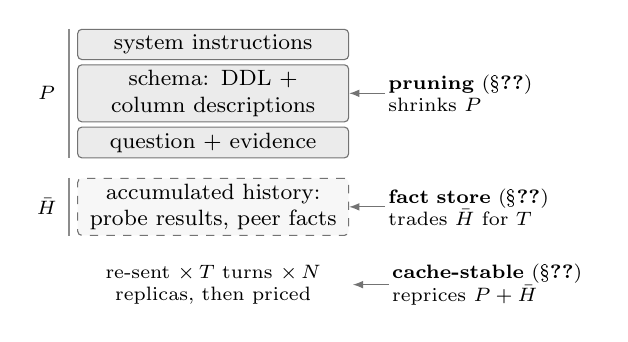
\begin{tikzpicture}[
  font=\footnotesize,
  bx/.style={draw=black!55, rounded corners=1.5pt, text width=3.3cm,
             align=center, minimum height=0.38cm, inner sep=2pt},
  frozen/.style={bx, fill=black!8},
  hist/.style={bx, fill=black!3, dashed, minimum height=0.72cm},
  note/.style={font=\scriptsize, align=left, text width=2.6cm, inner sep=1pt,
               anchor=west},
  arr/.style={-{Latex[length=1.3mm]}, black!55, thin}
]
\node[frozen]                      (sys)  {system instructions};
\node[frozen, below=1.5pt of sys]  (sch)  {schema: DDL + column descriptions};
\node[frozen, below=1.5pt of sch]  (task) {question + evidence};
\node[hist,   below=7pt   of task] (hst)  {accumulated history:\\probe results, peer facts};
\node[below=7pt of hst, font=\scriptsize, text width=3.3cm, align=center] (mul)
  {re-sent $\times\,T$ turns $\times\,N$ replicas, then priced};

\draw[black!45, line width=0.8pt]
  ([xshift=-3pt]sys.north west) -- ([xshift=-3pt]task.south west);
\draw[black!45, line width=0.8pt]
  ([xshift=-3pt]hst.north west) -- ([xshift=-3pt]hst.south west);
\node[font=\scriptsize] at ([xshift=-11pt]sch.west)  {$P$};
\node[font=\scriptsize] at ([xshift=-11pt]hst.west)  {$\bar{H}$};

% Anchored at each target's own height -> horizontal arrows.
\node[note] (m1) at ([xshift=13pt]sch.east)
  {\textbf{pruning} (§\ref{sec:prune})\\shrinks $P$};
\node[note] (m2) at ([xshift=13pt]hst.east)
  {\textbf{fact store} (§\ref{sec:p3})\\trades $\bar{H}$ for $T$};
\node[note] (m3) at ([xshift=13pt]mul.east)
  {\textbf{cache-stable} (§\ref{sec:pcache})\\reprices $P+\bar{H}$};

\draw[arr] (m1.west) -- (sch.east);
\draw[arr] (m2.west) -- (hst.east);
\draw[arr] (m3.west) -- (mul.east);
\end{tikzpicture}
\caption{Anatomy of one replica's prompt. The static prefix $P$ is re-sent
unchanged on every turn of every replica; the history $\bar{H}$ grows as the
episode proceeds. Each of the three methods attacks a different factor of
Eq.~\ref{eq:cost}.}
\label{fig:anatomy}
\end{figure}


\subsection{How much of that cost is wasted}\label{sec:waste}

Uncoordinated replication is expensive in exactly the way Eq.~\ref{eq:cost}
predicts. On the 50-task subset, moving from three replicas to twenty-five
raises duplicated exploratory SQL from 39--49\% to 76--89\% and total token
consumption from 3.1--3.5$\times$ to 26.6--36.7$\times$ that of the cheapest
correct replica, on all three models. Execution accuracy over the same range moves by at
most eight points, which is within the run-to-run variation of a 50-task subset,
so an eightfold increase in replicas buys an order of magnitude in cost and no
accuracy that can be distinguished from noise.

\subsection{Tokens consumed and tokens billed}\label{sec:ledgers}

Two quantities are reported separately throughout, because the results turn on
their difference. \emph{Raw tokens} are what the model consumed, and they are
what a content-level policy changes. \emph{Billed tokens} price that same
consumption with cached prefix tokens discounted at the provider's rate, and
they are what the user pays. A method that changes no content can move the
second without moving the first. Section~\ref{sec:results-pcache} reports a case
where the two move in opposite directions on one run, both significantly.
Execution accuracy is not a third ledger but a constraint, and nothing below is
reported as a saving unless accuracy survives it intact.

\section{Three ways to make the prompt cheaper}\label{sec:methods}

The cost identity of §\ref{sec:costmodel} exposes three distinct surfaces, and
the three methods evaluated here attack one each: schema pruning shrinks the
static prefix $P$, the semantic fact store reshapes the accumulated history $H$
against the turn count $T$, and cache-stable prompt structure changes the price
at which both are billed. Each is described below in the same four parts, covering what it changes,
the algorithm, its safety rails and failure mode, and how it composes. The
uniformity is deliberate, letting the designs be compared and not only their
results.

\subsection{Schema pruning: send a smaller schema}\label{sec:prune}

\textbf{What it changes.} Every turn re-sends the database schema, meaning the
DDL plus BIRD's column descriptions. Because that text sits in the static prefix, its
cost is multiplied by turns and again by replicas, even when the agent touches
two tables out of eight. Pruning trims the prefix once, before any replica
starts, so the saving applies to every subsequent billing event.

\textbf{Scoring.} Tables are scored against the question and evidence in one of
three modes, unified by \texttt{combined\_table\_scores}. The \emph{keyword}
mode tokenises the question and evidence and awards each table $+5$ where its
name appears as an exact token, $+3$ as a substring, $+2$ per column name
matching an exact token and $+1$ per column-name substring. The \emph{semantic}
mode builds a profile document per table, holding its name, the name split on
underscores, its column names, and every column description shipped with the
database. It then scores TF--IDF cosine similarity against the question, using
sublinear term frequency, smoothed inverse document frequency and $L_2$
normalisation. The implementation is self-contained, and no external embedding model
is involved, which keeps the step cheap enough to run per task. The
\emph{hybrid} mode, the default and the only one evaluated online here, averages
the two after max-normalising each.

\textbf{Selection.} Algorithm~\ref{alg:prune} gives the procedure, in which
seeds are drawn from tables carrying a non-zero \emph{keyword} score while the
continuous hybrid score orders candidates without by itself admitting them.
Those seeds are then expanded across the foreign-key graph, padded to a floor of
two tables, and finally passed through a set of per-database recall rules.

\begin{algorithm}[t]
\caption{Recall-aware hybrid schema pruning}\label{alg:prune}
\begin{algorithmic}[1]
\Require question $q$, evidence $e$, database $d$ with tables $\mathcal{T}$
\Ensure schema context over a subset of $\mathcal{T}$
\State $k \gets \textsc{KeywordScores}(q \Vert e, \mathcal{T})$
\State $s \gets \textsc{TfIdfCosine}(q \Vert e, \textsc{Profiles}(\mathcal{T}))$
\State $h \gets \tfrac{1}{2}\,\overline{k} + \tfrac{1}{2}\,\overline{s}$
  \Comment{max-normalised}
\State $S \gets \{t \in \mathcal{T} : k[t] > 0\}$
\If{$S = \emptyset$}
  \State $S \gets \{t : s[t] > 0\}$ \textbf{or} $\arg\max_t h[t]$ if
    $h[t] \geq \tau$
\EndIf
\If{$S = \emptyset$}
  \State \Return full schema
    \Comment{static fallback}
\EndIf
\State $S \gets S \cup \textsc{FkNeighbours}(S)$
\State $S \gets S \cup \textsc{TopUp}(h, S)$ \textbf{while} $|S| < 2$
\State $S \gets S \cup \textsc{RecallRules}(d, S)$
\If{$S = \mathcal{T}$} \State \Return full schema \EndIf
\State \Return DDL and column descriptions restricted to $S$
\end{algorithmic}
\end{algorithm}

\textbf{A worked example.} Question 1317 asks, of the \texttt{student\_club}
database, ``Among the students from the Student\_Club who attended the event
`Women's Soccer', how many of them want a T-shirt that's in medium size?''. The
gold query joins \texttt{event}, \texttt{attendance} and \texttt{member}. Only
two of the eight tables score on keywords, and the gold table
\texttt{attendance} scores exactly zero. The question names an event and a
garment, never the join table connecting them. It ranks third on the hybrid score, which is
not sufficient for admission, and enters the selection solely through the recall
rule that adds \texttt{attendance} whenever \texttt{event} is selected. The
result keeps three tables of eight and cuts the schema from 6{,}513 to 2{,}479
characters, a 61.9\% reduction, with gold-table coverage intact. The full score
table is Table~\ref{tab:appendix-prune-example}.

\textbf{Safety rails.} Two rails protect recall, and they differ in what they
cost. The \emph{static} fallback emits the full schema when nothing scores above
zero, and is free. The \emph{runtime} fallback restores the full schema after a
\texttt{no such table} execution error, and costs a turn. The runtime rail is
implemented twice, for one reason. The baseline loop rewrites the schema
message in place, whereas the cache-aware loop of §\ref{sec:pcache} folds the
restored schema into that turn's tool result instead, because rewriting the
prefix would invalidate the provider cache. The cached loop pays a turn to
protect the prefix. That is the first concrete instance of the tension
analysed in §\ref{sec:interact}.

\textbf{Failure mode.} A recall miss does more than forgo a saving, because it
sets the agent exploring blind and tokens rise. This was first seen during
development, when an earlier heuristic that missed gold tables on 10 of 50 tasks
increased token consumption by roughly 35\%, and §\ref{sec:results-prune} measures
the same effect at full scale and finds it larger still. Pruning that breaks
recall is worse than no pruning at all, which is why recall is treated below as
a precondition rather than a diagnostic.

\textbf{Known limits.} Foreign-key expansion is enabled for one database
only. In \texttt{student\_club} the key graph is fully connected, so expanding
across it would re-admit the whole schema and undo the prune. The recall rules
are likewise hand-written per database. Both are the reason the method's
generalisation is bounded, and §\ref{sec:results-prune} measures where that
bound falls.

\subsection{The fact store: share what replicas learn}\label{sec:p3}

\textbf{What it changes.} Where pruning shrinks what is sent once, the fact store
changes what accumulates. It trades additional bytes in $H$ for a reduction in
$T$: if a replica can read a peer's finding, it need not spend a turn
rediscovering it.

\textbf{Structure.} One store exists per task and is shared by that task's $N$
replicas under a single lock. It holds two maps. The first keys distilled facts on their
normalised text, and, for each fact, the set of replicas that discovered it
independently. The second map is what makes peer knowledge distinguishable from
a replica's own, and it is also what allows corroborated facts to be ranked
first.

\textbf{Write path.} After every exploratory query, and never after a
submission, the outcome is distilled by rules that make no model calls at all, so the
coordination layer adds no inference cost of its own and every token it costs is
prompt text. Queries are canonicalised by parsing them to an
abstract syntax tree with \texttt{sqlglot} (Mao 2024), so that two spellings of
one probe collapse to a single fact. The rules emit a normalised form of the
query itself,
up to two working join predicates, a row count, simple statistics over at most
three numeric columns, and, for small results, the distinct values of up to four
low-cardinality columns. An execution error short-circuits the rest and is
published as a fact in its own right.

\textbf{Read path.} Before each turn a replica requests the facts it did not
itself discover. These are ordered by the number of replicas that found them
independently, so corroborated findings surface first, and are then truncated to
at most eight bullets and 500 characters, with a guarantee of at least one fact.

\textbf{A worked example.} Question 1350 of \texttt{student\_club} asks ``What
is the status of the event which bought `Post Cards, Posters' on 2019/8/20?''.
Across ten replicas, 24 exploratory probes distil to 14 distinct facts, of which
one replica's digest receives seven. Both caps bind. That digest is reproduced
verbatim as Fig.~\ref{fig:appendix-digest}, and what the peers mostly report is
worth noting: joins that work, and probes that returned nothing. Negative
results are the store's most common payload, and they are genuinely useful,
since a peer that has established a join is empty saves another replica the same
query. They are also why the digest can grow without shortening any
trajectory.

\textbf{Two ways to add the digest.} How the digest reaches the prompt matters
more than it first appears. The baseline loop removes any previous digest from
the middle of the message list and appends a fresh one each turn. The
cache-aware loop instead appends only the facts a given replica has not yet
seen, tracked per replica, as a single trailing message, and never edits an
existing one. The second exists solely so that this method and the next can
coexist. Section~\ref{sec:pcache} explains why the first would make the third method
inert.

\textbf{Failure mode.} The digest is advisory, presented as context that the
model remains free to ignore. What the design cannot control is the balance of
two opposing terms. The injection is paid on every turn of every replica and
grows with $N$, because more replicas publish more facts. The saving depends on
whether reading a fact actually removes a probe. Nothing in the mechanism
determines which term wins, and §\ref{sec:results-p3} finds the answer is a
property of the model rather than of the configuration.

\textbf{A known limit.} The store caps at 128 entries with no eviction,
so once it is full new facts are silently dropped, and although the cap is
rarely reached on the tasks studied here it remains a real ceiling on longer
trajectories.

\subsection{Cache-stable structure: pay less for the same bytes}\label{sec:pcache}

\textbf{What it changes.} Neither preceding method touches the rate at which
tokens are billed. Providers discount input that repeats a previously seen
prefix, which makes the price of $P + H$, rather than their size, a third and
independent lever. Nothing here is stored locally. The mechanism is entirely a
matter of presenting the prompt so that the provider's own cache can fire.

\textbf{Two invariants.} Provider prefix caches share two requirements. The
cached span must be byte-identical from the first token, and it may only grow by
appending. The baseline loop violates both. Peer-context injection removes and
re-appends a message in the middle of the list every turn, which shifts
everything after the schema and collapses the stable prefix to the system
message and the task, and the pruning runtime fallback rewrites the schema message
in place. A third problem is subtler still: no backend recorded the provider's
cached-token counts, so even a cache that did fire would have been invisible in
the results.

\textbf{Three zones.} The cache-aware loop partitions the prompt instead, and
Fig.~\ref{fig:zones} contrasts the two message lists. Zone~1 holds the system
message and the task message carrying the schema, question and evidence, and it
is built once and never mutated. Zone~2 is append-only, so peer context arrives as
deltas, and the pruning fallback folds a restored schema into the trailing tool
result rather than splicing the prefix. An optional Zone~3 carries a single
volatile trailer. Cached-token counts are read from each provider's usage
metadata and recorded per turn, which is what makes the billing ledger of
§\ref{sec:results-pcache} measurable at all.

\begin{figure}[t]
\footnotesize\ttfamily\raggedright
\textbf{\rmfamily Baseline loop, turn $n$:}\\
{[}0{]} system\\
{[}1{]} task + schema \quad\textrm{\itshape (rewritten by fallback)}\\
{[}2{]} \ldots history \ldots\\
{[}k{]} peer context \quad\textrm{\itshape (removed, re-appended: shifts $k{+}1$ on)}\\[4pt]
\textbf{\rmfamily Cache-aware loop, turn $n$:}\\
{[}0{]} system \quad\textrm{\itshape (frozen)}\\
{[}1{]} task + schema \quad\textrm{\itshape (frozen)}\\
{[}2{]} \ldots history, append-only \ldots\\
{[}n{]} new peer facts only \quad\textrm{\itshape (appended)}
\normalfont\rmfamily
\caption{Why the baseline loop cannot cache. Re-appending peer context mutates
the interior of the message list, so no prefix beyond the first two messages is
byte-stable across turns.}
\label{fig:zones}
\end{figure}

\textbf{Safety.} This method is accuracy-neutral by construction. Not one
content byte differs between the two loops, only the order and stability of the
messages carrying it. That claim is enforced, not merely asserted: a unit test
simulates five turns of injections and tool results, then checks that the first
two messages remain byte-identical throughout. Its failure mode is also
benign. If an invariant is broken the cache silently stops firing and cost
returns to baseline. Nothing becomes incorrect. This distinguishes it from the
two preceding methods, whose failure modes change what the model sees.

\textbf{Why the saving is this large.} The size of the billing saving is set as much by
the provider's price list as by the mechanism. Cached input costs 50\% of the
standard input rate on GPT-4o mini, 10\% on Gemini 2.5 Flash and 2\% on
DeepSeek, so the identical mechanism is worth twenty-five times more on one
provider than another. Section~\ref{sec:results-pcache} reports all three, and
the spread between them should be read as a pricing fact rather than a property
of the method.

\subsection{How the three methods interact}\label{sec:interact}

Composed, the three methods interact through three channels, and they do not
point the same way.

The channel most easily anticipated is \emph{substitutive}: pruning removes
schema bytes that the cache would otherwise have served at a discount, so the
two savings overlap and the stack should recover less than the sum of its parts.
The second is \emph{enabling}: the delta-based injector of §\ref{sec:p3} exists
only so that shared knowledge can be added without breaking the prefix, so
without it the combination would not merely underperform but would disable the
third method outright. The third is \emph{complementary}: against a pruned
prefix, distilled facts may substitute for schema the pruner discarded, in which
case the digest stops being pure overhead and begins to carry information the
model would otherwise have gone looking for.

The first channel predicts a stack that underperforms its components, the third
one that exceeds them. Which dominates is an empirical question, and
§\ref{sec:results-compose} measures it.

\section{How the experiments were run}\label{sec:setup}

\textbf{Data, models and configuration.} All experiments run on BIRD mini-dev
over its eleven SQLite databases, with the gold evidence annotations included in
the prompt as the benchmark intends. Three API models are used, GPT-4o mini,
Gemini 2.5 Flash and DeepSeek v4-flash, at temperature 0 with
\texttt{best\_of\_n} coordination and a 15-turn cap. Each method of
§\ref{sec:methods} is evaluated alone, and all three together, against a matched
uncoordinated baseline.

\textbf{How the coverage is split.} Coverage is split deliberately, not uniformly. On a
50-task subset the full grid runs at $N \in \{3, 10, 25\}$, giving four arms by
three models by three replica counts for thirty-six cells, while on the full
500-task split the same four arms run at $N \in \{3, 10\}$ and add twenty-four
more. Sixty cells in all. Spending the larger budget on tasks instead of a third replica count
follows from the accuracy constraint. At fifty tasks the paired interval on an
execution-accuracy difference has a median half-width of $\pm$7.0 percentage
points, so ``no accuracy cost'' can only mean ``a seven-point loss cannot be
ruled out''. That is too weak to carry a paper whose central claim is that cost
falls while accuracy does not. At roughly 500 matched tasks the same interval
tightens to $\pm$2.4 points. Only $N = 25$ is therefore subset-only, and
§\ref{sec:results-p3} shows what the choice bought: one 50-task result reverses
outright at full scale.

\textbf{Isolation.} No policy outside the three under study is enabled in any
arm. There is no early stopping, no shared execution cache, and no suppression of
repeated probes, so the composed arm is exactly these three methods and each
isolated arm differs from its baseline in exactly one respect. This is
stricter than such layers are usually reported, and §\ref{sec:results-compose}
shows why it matters: a component that looks worthless measured alone turns out
to earn its place in the stack.

\textbf{Metrics and statistics.} Five quantities are reported per cell:
execution accuracy, raw prompt and completion tokens, the share of input served
from the provider cache, billed tokens with cached input priced at each
provider's published cached rate, and digest injections per task for arms that
include the fact store. All comparisons are paired. The intersection of completed
\texttt{question\_id}s is taken, a per-question difference vector formed, and
that vector resampled with replacement 10{,}000 times under a fixed seed to give
a percentile 95\% interval. Token ratios are bootstrapped as a ratio of
resampled sums, not as a mean of per-task ratios, so that a few cheap tasks
cannot dominate. Throughout, $\dag$ marks an interval containing zero, and no
effect is claimed for such a cell. Batches completing under 90\% of their tasks
are refused outright.

\textbf{Scope.} Two limits belong here rather than in the discussion. The design
is complete at both scales for all four arms, but $N = 25$ was measured only on
the subset, so every claim about behaviour at twenty-five replicas rests on
fifty tasks. And no cell is replicated on a second seed, which means run-to-run
variation is bounded by the reported intervals and not by repetition. This paper also narrows the scope registered in its project definition, which
named five policies across the execution and prompt layers. The two
execution-layer policies are omitted because their contribution could not be
attributed cleanly when measured inside a stack.

\section{Results}\label{sec:results}

\subsection{Does a smaller schema pay?}\label{sec:results-prune}

On the 50-task subset, pruning looks like the most dependable lever in the
study. Raw tokens fall in all nine configurations by 14.7--28.7\%, eight of the
nine intervals exclude zero, and no accuracy interval does. Nor does the saving
decay as replicas are added. It is largest at $N = 25$, reaching $-$28.7\%
on GPT-4o mini and $-$24.8\% on Gemini, exactly as Eq.~\ref{eq:cost} predicts of
a term re-billed on every turn of every replica
(Table~\ref{tab:appendix-matrix-50}).

At full scale that result largely disappears. Across all 500 tasks at $N = 3$,
isolated pruning saves $-$8.5\% on GPT ([$-$16.6, $+$0.9]), $-$3.9\% on Gemini
([$-$11.9, $+$4.8]) and $-$3.0\% on DeepSeek ([$-$11.8, $+$6.9]). Not one
interval excludes zero. At $N = 10$ the same measurement partly recovers:
$-$10.9\% on GPT ([$-$17.6, $-$3.2]) and $-$9.1\% on DeepSeek ([$-$15.5,
$-$1.8]) both exclude zero, while Gemini reaches $-$8.3\% on an interval that
misses by a tenth of a point ([$-$15.8, $+$0.1]). A method that does nothing at three replicas and something at ten is not a
method whose headline number means much, and the offline analysis explains why
the aggregate is the wrong object of study in the first place.
On the smoke subset the pruner retains every gold table on every task, and across
the full split it does so for 448 of the 500, or 89.6\%, because the recall rules
of §\ref{sec:prune} are written per database and eleven databases are not eleven
rules. Splitting the full-scale runs on that offline signal separates two
populations the aggregate had been averaging together
(Table~\ref{tab:recall-split}): a 9.9--19.7\% saving where recall is complete,
and a 32--156\% \emph{increase} where a gold table is missing. The regimes are
stable where the aggregate is not.

\begin{table}[t]
\caption{Isolated pruning at full scale, split by whether the offline analysis
retained every gold table for that question. Paired bootstrap 95\% intervals on
raw tokens, in per cent; \dag\ marks an interval containing zero. Recall-complete
groups hold 440--446 questions, recall-incomplete groups 38--50. Every
recall-complete cell saves significantly and every recall-incomplete cell costs,
and the split is the same at both replica counts.}
\label{tab:recall-split}
\centering
\scriptsize
\begin{tabular}{@{}llrr@{}}
\toprule
 & & \multicolumn{2}{c}{Raw-token change (\%)} \\
\cmidrule(l){3-4}
$N$ & Model & Recall complete & Recall incomplete \\
\midrule
3 & GPT-4o mini & $-$16.1 [$-$21.6, $-$10.3] & $+$55.3 [$-$0.6, $+$139.7]\dag \\
3 & Gemini 2.5 Flash & $-$19.4 [$-$23.1, $-$15.6] & $+$155.8 [$+$87.2, $+$230.8] \\
3 & DeepSeek v4-flash & $-$9.9 [$-$17.9, $-$0.8] & $+$57.4 [$+$21.5, $+$110.1] \\
\midrule
10 & GPT-4o mini & $-$17.8 [$-$22.1, $-$13.4] & $+$49.7 [$-$2.0, $+$123.3]\dag \\
10 & Gemini 2.5 Flash & $-$19.7 [$-$23.7, $-$15.3] & $+$137.2 [$+$55.8, $+$230.4] \\
10 & DeepSeek v4-flash & $-$13.8 [$-$20.5, $-$5.9] & $+$32.1 [$+$13.2, $+$56.3] \\
\bottomrule
\end{tabular}
\end{table}

A missed table therefore does more than forfeit the saving: it multiplies the
cost, because an agent handed a schema without a table it needs does not fail
quickly but explores, retries, and on Gemini spends more than two and a half
times what the unpruned run spends on the same question. One task in ten behaving that
way cancels the saving on the other nine, which yields a deployment rule with a
test attached. Which regime a task falls into is knowable \emph{before any model
is called}, because offline gold-table recall needs no inference, only the gold
queries, and it predicts the sign of the token effect. Validate it per database,
enable pruning where recall is complete, and treat anything short of complete
recall as a blocker for that database. Correctness of table selection, not
aggressiveness of reduction, decides whether shrinking the prefix pays at all.

The shortfall is concentrated rather than diffuse, since the four databases
carrying
hand-written recall rules retain every gold table, while \texttt{financial} and
\texttt{california\_schools}, which carry none, retain them on 56\% and 60\% of
tasks and account for most of the misses. Reduction and recall are not in
tension, since the most aggressively pruned database, \texttt{student\_club} at
62.5\%, keeps every gold table. The per-database breakdown is
Table~\ref{tab:appendix-perdb}.

\subsection{Does the fact store pay on its own?}\label{sec:results-p3}

Measured in isolation, the fact store is the least predictable of the three
methods, and the only one whose direction depends on how many tasks it is
measured over.

On the 50-task subset its token effect has no consistent sign. GPT-4o mini saves
17.2\% at three replicas, Gemini is indistinguishable from zero at every replica
count, and DeepSeek \emph{pays}, at 20.2\%, 21.1\% and 16.0\% for three, ten and
twenty-five replicas, two of the three intervals excluding zero. Read on its own
that is a clean per-model result, and it invites a mechanical explanation. The
store taxes every turn of every replica with injected text. Injections per task
grow steeply with $N$, from 6.0 to 52.6 on GPT and 10.2 to 89.4 on DeepSeek, and
whether the method pays turns on whether saved probes outrun that tax.

The full split contradicts it. Across all 500 tasks the fact store saves 8.9\%
and 8.8\% on GPT at three and ten replicas, both intervals excluding zero.
Gemini remains null, and DeepSeek, the model that appeared to pay most,
\emph{saves} 5.8\% and 7.0\%, significantly at ten replicas. Four of the six
full-scale cells save, three of them significantly, and none pay, as the
complete grid in Table~\ref{tab:appendix-matrix-500} shows.

The injection tax cannot explain the reversal, because the tax barely moved:
DeepSeek carries 32.4 injections per task at fifty tasks and 28.3 at five
hundred, for the same ten replicas. What changed is the sample. The subset
over-represents tasks on which peer facts are redundant, and the tax that looked
decisive is better described as a quantity that \emph{bounds} the saving than
one that predicts its sign. This is the clearest instance in the study of a
50-task result that does not survive scale, and it is a caution about the subset
sizes at which coordination layers are usually evaluated.

Accuracy is where the method's real cost appears. On DeepSeek at full scale and
ten replicas the fact store saves 7.0\% of tokens while losing 3.5 points of
execution accuracy ([$-$5.7, $-$1.4]), which is the only cell in the entire
design where a method in isolation moves accuracy at all, as
§\ref{sec:results-ex} sets out. Everywhere else the store is accuracy-neutral, and
nowhere does it improve accuracy. Shared knowledge is advisory, and a replica
that adopts a peer's premature finding can be led away from a correct
trajectory as easily as toward one.

\subsection{Does cache-stable structure pay?}\label{sec:results-pcache}

Unconditionally, and by the largest margin in the study. Cache-stable structure
is the only method here that changes no content: the bytes sent are identical to
the baseline's, reordered only so that the prefix stays stable and growth
remains append-only. What changes is the rate at which they are billed.

The prediction is unusually sharp and falsifiable in two directions at once:
raw consumption should not move, while billed input should fall by whatever
share of the prompt the provider serves from cache. Across the fifteen measured
configurations, raw tokens are indistinguishable from zero in fourteen, while
billed input falls in \emph{all} fifteen, from 18.8\% to 86.0\%, every interval
excluding zero.


The full-scale half of that grid is the cleanest evidence in the paper for the
two-ledger claim of §\ref{sec:ledgers}: six cells in which one ledger does not
move while the other falls from $-$38.3\% on GPT-4o mini to $-$86.0\% on
DeepSeek. Fig.~\ref{fig:twoledger} shows that
separation across the whole design, with the methods that change content lying
along the diagonal and the method that changes only price falling far below it.
The complete grids, with intervals, are
Tables~\ref{tab:appendix-matrix-50} and~\ref{tab:appendix-matrix-500}.

The single cell that breaks raw-token neutrality is worth reporting rather than
rounding away. On the 50-task subset at $N = 10$, GPT-4o mini records raw
$+$10.2\% [$+$0.6, $+$24.0] against billed $-$18.8\% [$-$26.6, $-$8.8]: the same
run, both intervals excluding zero, the two ledgers moving in opposite
directions. This is not a mechanism effect, because a method that changes no
content cannot make an agent consume more. It is the expected consequence of a
design that is content-neutral \emph{per turn} yet not trajectory-identical: a
reordered prompt can still tip a sampled decision. The full-scale measurement
settles it, recording raw $+$1.9\% [$-$0.7, $+$4.7] on ten times the sample. The
excursion was subset noise, and the billed comparison was the meaningful one
throughout.

The per-turn cache shares show the mechanism directly. DeepSeek serves 94--97\%
of input from cache from the first turn, while GPT-4o mini climbs from 53\% at the
first turn to roughly 80\% by the fourth, as an append-only history accumulates
behind a frozen prefix. That climb is the cost identity read backwards. The
longer the conversation runs, the larger the share of $P + \bar{H}$ already
seen, and the more of it the provider discounts.

Two qualifications belong with the result. First, the spread across models is a price schedule as much as a mechanism,
since DeepSeek's 86\% is mostly its 50-fold cached discount and an identical hit
rate would be worth 40\% on GPT. Second,
provider caches are opaque and cached-token counts are provider-reported. This
work takes both at face value and prices them at published list rates.

\begin{figure}[t]
\centering

\includegraphics[width=\columnwidth]{figures/fig4_two_ledger.png}
\caption{Raw against billed token change for all sixty measured cells. Colour is
the model, shape the method. Filled markers are the 50-task subset and open
markers the 500-task split. The dashed line marks raw $=$ billed. Pruning and
fact-store cells track it, because they change content and so move both ledgers
together, while prompt-cache and composed cells fall far below it. Every
DeepSeek cell carrying the cache sits on a floor near $-$85\%. The labelled cell is the
one that moves in opposite directions on the two ledgers, both intervals
excluding zero.}
\label{fig:twoledger}
\end{figure}


\subsection{Do the three add up when combined?}\label{sec:results-compose}

Because the three methods act on different factors of Eq.~\ref{eq:cost}, their
savings would compose multiplicatively if they did not interact. That product is
the null tested here. For each of the fifteen configurations the isolated arms
give a predicted change and the composed arm a measured one, and the gap between
them is the interaction.

The stack beats that prediction in eleven of fifteen configurations. The
clearest case is DeepSeek at three replicas on
the subset, where the parts predict a net \emph{increase} of 8.3\%, the fact
store's 20.2\% penalty outweighing pruning's 14.7\% saving. The composed stack
removes 23.8\% instead, a gap of 32 points. Two of the three interaction
channels of §\ref{sec:interact} predict exactly this: distilled peer facts
substitute for schema the pruner removed, and the append-only injection
discipline lets the fact store coexist with the cache instead of invalidating
it. The four configurations that miss do so narrowly, and none reverses: GPT
falls 7.4 and 3.6 points short at three and twenty-five replicas on the subset,
and at full scale with ten replicas Gemini and DeepSeek come within 2.1 and 0.3
points of the null. In no configuration does the stack save appreciably less
than its parts.


Two cautions constrain how far that can be pushed. The comparison is
descriptive, not inferential:
isolated and composed cells come from independent runs rather than paired ones,
so no interval attaches to a gap, and eleven of fifteen in one direction is a
tendency rather than a tested effect. And the tendency is strongest where the
evidence is weakest. The four misses concentrate at full scale, where intervals
are tightest, while the widest super-additive gaps all sit at fifty tasks. The defensible claim is that composition at least matches, and usually
exceeds, the product of its parts, with the excess largest at small $N$.

The deployment consequence is the reason this matters.
Section~\ref{sec:results-p3} found the fact store had no reliable sign alone and
cost accuracy on one model, so an ablation stopping there would drop it. Yet it is
a component of every composed configuration measured here, including the two
that save most. Isolation is necessary to attribute a saving to a mechanism. It
is not sufficient to decide whether that mechanism belongs in the stack, and a
study that reported only isolated ablations would recommend removing a component
that pays for itself in company.

\subsection{Does accuracy hold throughout?}\label{sec:results-ex}

Across all sixty measured cells, fifty-eight execution-accuracy intervals
contain zero. Sixty intervals at 95\% confidence would be expected to
produce roughly three exceptions if no method affected accuracy anywhere, so two
is fewer than chance alone would give.

That arithmetic is not the whole answer, because the two exceptions are not
independent draws. Both are DeepSeek at full scale and ten replicas, the fact
store alone at $-$3.5 points and the composed stack at $-$2.4 points. The two
arms at that same cell that do \emph{not} contain the fact store are both
consistent with zero, pruning at $-$1.6 and prompt cache at $-$1.2. A pair of exceptions
sharing a model, a cell and a mechanism is weaker evidence of coincidence than a
scattered pair would be. The constraint holds across the design as a whole,
and it is violated in one identified place by one identified component, as
§\ref{sec:results-p3} explains.

\section{Discussion}\label{sec:discussion}

\textbf{Two ledgers, not one.} The clearest methodological result here is that
raw and billed tokens must be reported separately. A method can leave
consumption untouched and still remove most of the bill, as cache-stable
structure does in fourteen of fifteen configurations. In one configuration the
two ledgers move in opposite directions, both intervals excluding zero.
A study reporting only raw tokens would have concluded that the single most
valuable method in this paper does nothing.

\textbf{Each method has a different ceiling.} Prefix reduction is bounded
by recall, and the bound is sharp, not gradual. The same pruner saves on tasks
whose gold tables survive and costs several times as much where one does not.
What limits the method is how reliably the right tables are kept, not how
aggressively the prefix can be cut, and hand-written per-database rules are
where that reliability runs out. History reshaping is bounded by something less
tractable. The injection tax is real and grows steeply with replica count, yet
it does not predict the sign. DeepSeek carries a near-identical load at both
scales while its token effect reverses, so the tax bounds the achievable saving
without determining it. Repricing is bounded only by the provider's cached
discount, which runs to 50\% of standard on GPT-4o mini, 10\% on Gemini and 2\%
on DeepSeek, and that is why it dominates and why one unchanged mechanism is
worth twice as much on one provider as on another. The ceiling sits entirely outside the
system.

\textbf{What isolation shows, and what it misses.} Attribution and deployment
are different questions, and the fact store answers them differently. Measured alone it has
no reliable sign, and on one model at full scale it costs accuracy. An ablation stopping
there would remove it. Yet it appears in every composed configuration measured,
including those that save most, and the composed stack beats the
product of its parts in eleven of fifteen configurations. Isolation is necessary to attribute a saving to a mechanism and insufficient to
decide whether that mechanism belongs in a deployment, which yields a
transferable rule: report both, and never let an isolated null veto a component
that pays in company.

\textbf{Positioning.} Schema linking and prompt compression pursue the same
reduction as §\ref{sec:prune}, but for a single pass. Multiplying by replicas
and turns is what makes a recall failure expensive instead of merely
regrettable. Role-based coordination such as MAC-SQL occupies an orthogonal
axis, and this layer would sit beneath it unchanged.

\textbf{Threats to validity.} Two limitations are structural. First, every cell
is a single run: the eleven-of-fifteen composition pattern is a consistent
direction across configurations, not a replicated effect, and breadth across
three models and two scales substitutes for depth. Second, coverage is uneven and the
two scales disagree twice, on pruning's aggregate and on the fact store's sign.
Where they disagree, the 50-task result is the one that fails, so subset
magnitudes should be read as indicative. Several narrower limits follow. The 89.6\% gold-table recall rests on
hand-written per-database rules and is a generalisation ceiling. The additivity
check compares independent runs against a \emph{multiplicative} null, so no
interval attaches to a gap. Provider caches are opaque, counts are
provider-reported, and prices are list rates checked on one date. Gold evidence
is included in prompts, as the benchmark intends, which flatters all arms
equally, and because no timing data was captured no latency claim appears
anywhere. And this paper
evaluates three of the five policies its registered definition named, a
narrowing forced by the isolation discipline above and declared openly. Finally, the
accuracy constraint is met in 58 of 60 cells but not in two, and those two share
a model, a cell and a mechanism instead of being scattered. That is weaker
evidence of coincidence than the count alone suggests, and it is why
§\ref{sec:results-p3} treats the effect as a property of the fact store.

\section{Conclusion and future work}\label{sec:conclusion}

A speculative agent re-sends its prompt on every turn of every replica, and the
identity $N \times T \times \mathrm{price}(P + \bar{H})$ has exactly three
factors to attack. Measuring one method against each, in isolation and composed,
across three models and sixty cells, gives a different answer for each factor.
Repricing is unconditional. Cache-stable structure changes no content byte,
leaves raw consumption unmoved in fourteen of fifteen configurations, and still
removes 18.8--86.0\% of billed input in all fifteen. Shrinking the prefix is
conditional on recall, and that condition is decidable offline before any model
runs. Pruning saves 9.9--19.7\% where every gold table survives and adds
32--156\% where one does not. Reshaping history pays only in company. Alone, the
fact store saves on two models of three at full scale but costs the third 3.5
points of accuracy, while the stack containing it beats the product of its parts
in eleven of fifteen configurations. Accuracy is unmoved in 58 of 60 cells.

What generalises furthest is not any of the three methods but the methodological
result behind them. Raw and
billed tokens are separate ledgers that can move in opposite directions in the
same run, and a policy must be judged on the one that binds. Isolation is
necessary to attribute an effect to a mechanism and insufficient to decide
deployment. The component this study is most critical of in isolation appears in
every configuration that saves most.

Four directions follow directly. Learned schema linking would lift the 89.6\%
recall ceiling without the hand-written per-database rules that currently set
it. The fact store needs eviction and a cost-aware injection budget, being
capped at 128 entries and silently dropping new keys once full, while the
injected digest grows with replica count unchecked. A paired, seeded
composed-versus-parts design would test the composition result inferentially
rather than descriptively, answering this paper's main statistical limitation,
while prefix persistence across tasks, gated against benchmark leakage, would
extend repricing beyond the single-task boundary it currently respects. Latency,
unmeasured here for want of instrumentation, remains the obvious complement to a
study of cost.

\section*{References}

\begingroup
\scriptsize
\setlength{\parindent}{0pt}

\refentry Anthropic (2024). \emph{Prompt Caching}. Anthropic API
documentation {[}online{]}. Available at: \url{https://docs.anthropic.com}
{[}Accessed 2 July 2026{]}.

\refentry Brown, B., Juravsky, J., Ehrlich, R., Clark, R., Le, Q., Ré, C. and
Mirhoseini, A. (2024). Large Language Monkeys: Scaling Inference Compute with
Repeated Sampling. \emph{arXiv preprint}.

\refentry Chen, L., Zaharia, M. and Zou, J. (2023). FrugalGPT: How to Use
Large Language Models While Reducing Cost and Improving Performance.
\emph{arXiv preprint}.

\refentry Gao, D., Wang, H., Li, Y., Sun, X., Qian, Y., Ding, B. and Zhou, J.
(2024). Text-to-SQL Empowered by Large Language Models: A Benchmark
Evaluation. \emph{Proceedings of the VLDB Endowment}, 17(5), 1132--1145.

\refentry Gim, I., Rajbhandari, S., Yao, Z., Aminabadi, R.Y., Rasley, J. and
He, Y. (2024). Prompt Cache: Modular Attention Reuse for Low-Latency
Inference. \emph{Proceedings of MLSys}.

\refentry Google DeepMind (2024). \emph{Context Caching}. Gemini API
documentation {[}online{]}. Available at: \url{https://ai.google.dev}
{[}Accessed 2 July 2026{]}.

\refentry Hayes-Roth, B. (1985). A Blackboard Architecture for Control.
\emph{Artificial Intelligence}, 26(3), 251--321.

\refentry Hong, S., Zheng, X., Chen, J., Cheng, Y., Wang, J., Zhang, C. et
al.~(2023). MetaGPT: Meta Programming for a Multi-Agent Collaborative
Framework. \emph{arXiv preprint}.

\refentry Jiang, H., Wu, Q., Lin, C.-Y., Yang, Y. and Qiu, L. (2023).
LLMLingua: Compressing Prompts for Accelerated Inference of Large Language
Models. In: \emph{Proceedings of EMNLP 2023}.

\refentry Lei, W., Ren, Y., Zhang, Y. et al.~(2020). Re-examining the Role of
Schema Linking in Text-to-SQL. In: \emph{Proceedings of EMNLP 2020}.

\refentry Li, J., Hui, B., Qu, G., Yang, J., Li, B., Li, B. et al.~(2023).
Can LLM Already Serve as a Database Interface? A Big Bench for Large-Scale
Database Grounded Text-to-SQLs. In: \emph{Advances in Neural Information
Processing Systems 36}.

\refentry Mao, T. and contributors (2024). \emph{sqlglot: Python SQL Parser
and Transpiler} {[}software{]}. Available at:
\url{https://github.com/tobymao/sqlglot} {[}Accessed 2 July 2026{]}.

\refentry OpenAI (2024). \emph{Prompt Caching}. OpenAI API documentation
{[}online{]}. Available at: \url{https://platform.openai.com/docs}
{[}Accessed 2 July 2026{]}.

\refentry Pourreza, M. and Rafiei, D. (2023). DIN-SQL: Decomposed In-Context
Learning of Text-to-SQL with Self-Correction. In: \emph{Advances in Neural
Information Processing Systems 36}.

\refentry Qin, Y., Liang, S., Ye, Y., Zhu, K., Yan, L., Lu, Y. et al.~(2023).
ToolLLM: Facilitating Large Language Models to Master 16000+ Real-World APIs.
\emph{arXiv preprint}.

\refentry Schick, T., Dwivedi-Yu, J., Dess\`{i}, R., Raileanu, R., Lomeli, M.,
Zettlemoyer, L., Cancedda, N. and Scialom, T. (2023). Toolformer: Language
Models Can Teach Themselves to Use Tools. \emph{Advances in Neural Information
Processing Systems 36}.

\refentry Scholak, T., Schucher, N. and Bahdanau, D. (2021). PICARD: Parsing
Incrementally for Constrained Auto-Regressive Decoding from Language Models.
\emph{Proceedings of EMNLP}.

\refentry Snell, C., Lee, J., Xu, K. and Kumar, A. (2024). Scaling LLM
Test-Time Compute Optimally Can Be More Effective than Scaling Model
Parameters. \emph{arXiv preprint}.

\refentry Talaei, S. et al.~(2024). CHESS: Contextual Harnessing for
Efficient SQL Synthesis. \emph{arXiv preprint}.

\refentry Wang, B., Ren, C., Yang, J., Liang, X., Bai, J., Chai, L. et
al.~(2025). MAC-SQL: A Multi-Agent Collaborative Framework for Text-to-SQL.
In: \emph{Proceedings of COLING 2025}.

\refentry Wang, B., Shin, R., Liu, X., Polozov, O. and Richardson, M. (2020).
RAT-SQL: Relation-Aware Schema Encoding and Linking for Text-to-SQL Parsers.
\emph{Proceedings of ACL}.

\refentry Wang, X., Wei, J., Schuurmans, D., Le, Q., Chi, E., Narang, S.,
Chowdhery, A. and Zhou, D. (2023). Self-Consistency Improves Chain of Thought
Reasoning in Language Models. In: \emph{Proceedings of ICLR 2023}.

\refentry Wooldridge, M. (2009). \emph{An Introduction to MultiAgent Systems}.
2nd edn. Chichester: John Wiley \& Sons.

\refentry Wu, Q., Bansal, G., Zhang, J., Wu, Y., Li, B., Zhu, E. et al.~(2023).
AutoGen: Enabling Next-Gen LLM Applications via Multi-Agent Conversation.
\emph{arXiv preprint}.

\refentry Yao, S., Zhao, J., Yu, D., Du, N., Shafran, I., Narasimhan, K. and
Cao, Y. (2023). ReAct: Synergizing Reasoning and Acting in Language Models.
In: \emph{Proceedings of ICLR 2023}.

\refentry Yu, T., Zhang, R., Yang, K., Yasunaga, M., Wang, D., Li, Z. et
al.~(2018). Spider: A Large-Scale Human-Labeled Dataset for Complex and
Cross-Domain Semantic Parsing and Text-to-SQL Task. In: \emph{Proceedings of
EMNLP 2018}.

\refentry Zhang, Y., Wang, B. and Yu, T. (2023). Benchmarking and Improving
Schema Linking for Text-to-SQL. In: \emph{Proceedings of EMNLP Findings}.

\refentry Zheng, B., Zhang, J., Mo, X., Liu, C. and Liu, Y. (2023). GPTCache:
An Open-Source Semantic Cache for LLM Applications. In: \emph{Proceedings of
NLP-OSS 2023}.

\refentry Zhong, R., Yu, T. and Klein, D. (2020). Semantic Evaluation for
Text-to-SQL with Distilled Test Suites. In: \emph{Proceedings of EMNLP 2020}.

\endgroup

\section*{Appendix}

\subsection*{Generative AI usage}

\scriptsize
Generative AI tools (Claude Code and Cursor agents) were used, under the
author's direction and review, for implementation assistance on the agent
harness and the three prompt-layer methods; for generation of intermediate
chapter drafts from experiment reports; and for editorial drafting of this paper
from those drafts. All quantitative content is computed by deterministic scripts
from JSONL execution traces. No figure or table value is model-generated, and
the tables in this appendix are emitted directly from the analysis outputs by
\texttt{make\_v8\_appendix\_tables.py}. All design decisions, result
interpretation and final text were reviewed and approved by the author;
AI-suggested references were verified against source records before inclusion.
\normalsize

\subsection*{Reproducibility}

\scriptsize
Source code, batch summaries, analysis reports and figure-generation scripts are
submitted with the paper, together with the complete JSONL traces of one
demonstration run so that the trace format can be inspected. Every quantitative
claim traces to a batch identifier
and a generating script, listed in Table~\ref{tab:appendix-repro}. Identifiers
follow the pattern \texttt{v8\_[arm]\_[scale]\_r[N]}, where scale is
\texttt{50t} or \texttt{500t} and $N \in \{3,10,25\}$ at 50 tasks and
$\{3,10\}$ at 500; the table lists the arm only. The analysis
is run in strict mode, meaning \texttt{analyze\_v8\_results.py} without
\texttt{-{}-allow-legacy}, so only batches carrying a clean \texttt{v8\_}
identifier are admitted and pre-v8 batches are refused rather than silently
reused (§\ref{sec:setup}). Batches completing under 90\% of their tasks are
likewise refused. Regenerating every number, figure and appendix table from the
submitted batch summaries is four commands, and needs neither the benchmark
databases nor any model call.
\normalsize

\begin{table}[t]
\caption{Claim to batch to script. All analysis is offline: no result in this
paper requires re-running the agents.}
\label{tab:appendix-repro}
\centering
\scriptsize
\begin{tabular}{@{}>{\raggedright\arraybackslash}p{1.75cm}>{\raggedright\arraybackslash}p{1.0cm}>{\raggedright\arraybackslash}p{4.3cm}@{}}
\toprule
Claim & Arm & Generating script \\
\midrule
Baselines (§\ref{sec:waste}) & \texttt{p0} &
\texttt{run\_v8\_cleanup.sh}, \texttt{run\_v8\_500t\_r3.sh},
\texttt{run\_v8\_500t\_r10.sh} \\
Pruning (§\ref{sec:results-prune}) & \texttt{prune} &
\texttt{run\_v8\_matrix.sh}, \texttt{run\_v8\_prune\_fill.sh} \\
Offline recall (§\ref{sec:results-prune}) & n/a &
\texttt{analyze\_schema\_pruning.py} \\
Fact store (§\ref{sec:results-p3}) & \texttt{p3} &
\texttt{run\_v8\_matrix.sh} \\
Prompt cache (§\ref{sec:results-pcache}) & \texttt{pc} &
\texttt{run\_v8\_matrix.sh}, \texttt{run\_v8\_cleanup.sh} \\
Composition (§\ref{sec:results-compose}) & \texttt{comp} &
\texttt{run\_v8\_matrix.sh}, \texttt{run\_v8\_500t\_r3.sh} \\
\midrule
All intervals & n/a & \texttt{analyze\_v8\_results.py} \\
Additivity, cell counts & n/a & \texttt{v8\_additivity.py} \\
Fig.~\ref{fig:twoledger} & n/a & \texttt{make\_v8\_figures.py} \\
Tables \ref{tab:appendix-matrix-50}--\ref{tab:appendix-perdb} & n/a &
\texttt{make\_v8\_appendix\_tables.py} \\
\bottomrule
\end{tabular}
\end{table}

\subsection*{Worked examples}

The two examples of §\ref{sec:methods} in full. Both are reproduced from live
runs rather than reconstructed.

\begin{table}[h]
\caption{Hybrid pruning on question 1317 (§\ref{sec:prune}). Gold tables in
bold. Seeds are drawn from non-zero keyword scores, so the third gold table,
which the question never names, is admitted only by the recall rule.}
\label{tab:appendix-prune-example}
\centering
\footnotesize
\begin{tabular}{@{}lrrl@{}}
\toprule
Table & Keyword & Hybrid & Admitted by \\
\midrule
\textbf{event}      & 8 & 0.780 & seed \\
\textbf{member}     & 3 & 0.688 & seed \\
\textbf{attendance} & 0 & 0.329 & recall rule \\
budget              & 0 & 0.216 & \\
major               & 0 & 0.164 & \\
expense             & 0 & 0.153 & \\
income              & 0 & 0.123 & \\
zip\_code           & 0 & 0.089 & \\
\bottomrule
\end{tabular}
\end{table}

\begin{figure}[h]
\centering
\fbox{\begin{minipage}{0.93\columnwidth}
\footnotesize\ttfamily\raggedright
Shared semantic facts from parallel replicas on this task (reuse these instead
of re-probing):\\[2pt]
- budget/event/expense returned 0 row(s)\\
- explored: select e.status from expense as ex join budget as b on
  ex.link\_to\_budget = b.budget\_id join event as e on b.link\_to\_even\ldots\\
- join works: b.link\_to\_event = e.event\_id\\
- join works: ex.link\_to\_budget = b.budget\_id\\
- budget/expense returned 0 row(s)\\
- explored: select ex.expense\_id, ex.expense\_description, ex.expense\_date,
  b.link\_to\_event from expense as ex join budget as b on ex\ldots\\
- expense returned 0 row(s)
\end{minipage}}
\caption{The peer digest served to one replica on question 1350 of
\texttt{student\_club} (§\ref{sec:p3}), reproduced verbatim. Seven bullets and
500 characters of fact text: both caps bind. Five of the seven report a negative
result.}
\label{fig:appendix-digest}
\end{figure}

\subsection*{Complete results}

\scriptsize
Section~\ref{sec:results} reports summary rows. The full matrix follows: every
measured cell, all three ledgers, with paired bootstrap intervals.
Table~\ref{tab:appendix-perdb} breaks the offline pruning analysis down by
database, which is where the shortfall between smoke-subset and full-scale
recall becomes legible. The databases carrying hand-written recall rules retain
every gold table, and those without account for almost all of the misses.
\normalsize

% Generated by scripts/make_v8_appendix_tables.py -- do not edit by hand.
% Re-run after any change to runs/reports/v8_numbers.txt.
\begin{table*}[t]
\caption{Complete 50-task subset matrix: every measured cell against its matched
baseline, with paired bootstrap 95\% confidence intervals.
\dag{} marks an interval containing zero.}
\label{tab:appendix-matrix-50}
\centering\footnotesize
\begin{tabular}{@{}llrrlrlrl@{}}
\toprule
Method & Model & $N$ & \multicolumn{2}{c}{EX $\Delta$ (pp)} & \multicolumn{2}{c}{Raw tokens} & \multicolumn{2}{c}{Billed tokens} \\
\cmidrule(lr){4-5}\cmidrule(lr){6-7}\cmidrule(lr){8-9}
 & & & value & 95\% CI & value & 95\% CI & value & 95\% CI \\
\midrule
Schema pruning & GPT-4o mini & 3 & +2.0 & [$-$6.0, +10.0]\dag{} & $-$25.8\% & [$-$43.3, $-$2.3] & $-$24.3\% & [$-$41.1, $-$0.2] \\
 & GPT-4o mini & 10 & +4.0 & [$-$4.0, +12.0]\dag{} & $-$19.2\% & [$-$39.0, +10.1]\dag{} & $-$16.0\% & [$-$35.8, +12.2]\dag{} \\
 & GPT-4o mini & 25 & +6.0 & [$-$2.0, +14.0]\dag{} & $-$28.7\% & [$-$41.1, $-$9.1] & $-$25.7\% & [$-$38.2, $-$6.1] \\
 & Gemini 2.5 Flash & 3 & +4.0 & [$-$4.0, +12.0]\dag{} & $-$22.6\% & [$-$31.0, $-$13.7] & $-$16.7\% & [$-$25.0, $-$8.0] \\
 & Gemini 2.5 Flash & 10 & $-$2.0 & [$-$10.0, +6.0]\dag{} & $-$22.1\% & [$-$30.8, $-$13.1] & $-$16.1\% & [$-$24.4, $-$7.8] \\
 & Gemini 2.5 Flash & 25 & $-$2.0 & [$-$10.0, +6.0]\dag{} & $-$24.8\% & [$-$32.2, $-$16.8] & $-$19.6\% & [$-$26.2, $-$13.1] \\
 & DeepSeek v4-flash & 3 & $-$6.0 & [$-$14.0, +0.0]\dag{} & $-$14.7\% & [$-$26.2, $-$2.7] & $-$14.1\% & [$-$25.3, $-$2.2] \\
 & DeepSeek v4-flash & 10 & $-$2.0 & [$-$6.0, +0.0]\dag{} & $-$20.2\% & [$-$27.4, $-$12.2] & $-$19.3\% & [$-$26.5, $-$11.3] \\
 & DeepSeek v4-flash & 25 & +0.0 & [+0.0, +0.0]\dag{} & $-$18.8\% & [$-$27.3, $-$9.6] & $-$18.1\% & [$-$26.4, $-$8.9] \\
\midrule
Fact store & GPT-4o mini & 3 & $-$2.0 & [$-$6.0, +0.0]\dag{} & $-$17.2\% & [$-$29.8, $-$0.7] & $-$17.5\% & [$-$29.6, $-$1.3] \\
 & GPT-4o mini & 10 & $-$4.0 & [$-$10.0, +0.0]\dag{} & +0.9\% & [$-$21.4, +30.5]\dag{} & +1.5\% & [$-$20.8, +30.7]\dag{} \\
 & GPT-4o mini & 25 & $-$6.0 & [$-$14.0, +2.0]\dag{} & $-$13.2\% & [$-$29.7, +6.2]\dag{} & $-$11.8\% & [$-$28.7, +8.1]\dag{} \\
 & Gemini 2.5 Flash & 3 & +0.0 & [$-$8.0, +8.0]\dag{} & +1.9\% & [$-$8.0, +11.9]\dag{} & +1.1\% & [$-$7.3, +9.5]\dag{} \\
 & Gemini 2.5 Flash & 10 & +2.0 & [+0.0, +6.0]\dag{} & +8.4\% & [$-$0.7, +19.6]\dag{} & +7.2\% & [$-$1.2, +17.5]\dag{} \\
 & Gemini 2.5 Flash & 25 & +2.0 & [+0.0, +6.0]\dag{} & +3.4\% & [$-$4.7, +11.9]\dag{} & +2.9\% & [$-$4.2, +10.3]\dag{} \\
 & DeepSeek v4-flash & 3 & $-$6.0 & [$-$14.0, +0.0]\dag{} & +20.2\% & [+0.6, +39.2] & +19.7\% & [$-$0.0, +39.2]\dag{} \\
 & DeepSeek v4-flash & 10 & $-$4.1 & [$-$10.2, +0.0]\dag{} & +21.1\% & [$-$4.7, +47.3]\dag{} & +21.6\% & [$-$5.0, +49.3]\dag{} \\
 & DeepSeek v4-flash & 25 & +2.0 & [+0.0, +6.0]\dag{} & +16.0\% & [+0.8, +30.9] & +14.6\% & [$-$0.3, +29.1]\dag{} \\
\midrule
Prompt cache & GPT-4o mini & 3 & +6.0 & [+0.0, +14.0]\dag{} & $-$13.3\% & [$-$32.4, +5.6]\dag{} & $-$36.5\% & [$-$49.9, $-$21.1] \\
 & GPT-4o mini & 10 & +2.0 & [$-$4.0, +10.0]\dag{} & +10.2\% & [+0.6, +24.0] & $-$18.8\% & [$-$26.6, $-$8.8] \\
 & GPT-4o mini & 25 & $-$2.0 & [$-$6.0, +0.0]\dag{} & $-$1.5\% & [$-$10.4, +7.6]\dag{} & $-$28.0\% & [$-$34.5, $-$20.2] \\
 & Gemini 2.5 Flash & 3 & +0.0 & [$-$6.0, +6.0]\dag{} & +2.8\% & [$-$1.6, +8.5]\dag{} & $-$35.9\% & [$-$43.4, $-$27.1] \\
 & Gemini 2.5 Flash & 10 & $-$2.0 & [$-$6.0, +0.0]\dag{} & $-$0.6\% & [$-$3.7, +1.9]\dag{} & $-$45.3\% & [$-$49.5, $-$40.5] \\
 & Gemini 2.5 Flash & 25 & +0.0 & [+0.0, +0.0]\dag{} & +1.4\% & [$-$0.1, +3.2]\dag{} & $-$44.7\% & [$-$48.8, $-$40.1] \\
 & DeepSeek v4-flash & 3 & +0.0 & [+0.0, +0.0]\dag{} & +5.6\% & [$-$6.6, +20.9]\dag{} & $-$81.9\% & [$-$84.2, $-$79.2] \\
 & DeepSeek v4-flash & 10 & $-$2.0 & [$-$6.0, +0.0]\dag{} & +4.8\% & [$-$0.3, +10.9]\dag{} & $-$81.5\% & [$-$83.1, $-$79.9] \\
 & DeepSeek v4-flash & 25 & +0.0 & [+0.0, +0.0]\dag{} & $-$0.3\% & [$-$4.6, +4.2]\dag{} & $-$82.0\% & [$-$83.2, $-$80.7] \\
\midrule
Composed & GPT-4o mini & 3 & +6.0 & [$-$2.0, +14.0]\dag{} & $-$39.3\% & [$-$59.0, $-$11.3] & $-$47.1\% & [$-$63.8, $-$23.9] \\
 & GPT-4o mini & 10 & +0.0 & [$-$8.0, +8.0]\dag{} & $-$29.5\% & [$-$43.9, $-$7.6] & $-$37.4\% & [$-$48.9, $-$20.2] \\
 & GPT-4o mini & 25 & $-$2.0 & [$-$10.0, +6.0]\dag{} & $-$35.4\% & [$-$47.4, $-$18.7] & $-$43.9\% & [$-$53.5, $-$30.3] \\
 & Gemini 2.5 Flash & 3 & +0.0 & [$-$8.0, +8.0]\dag{} & $-$23.6\% & [$-$32.8, $-$13.1] & $-$23.4\% & [$-$31.8, $-$13.9] \\
 & Gemini 2.5 Flash & 10 & $-$6.0 & [$-$14.0, +2.0]\dag{} & $-$24.6\% & [$-$33.5, $-$14.5] & $-$32.0\% & [$-$38.1, $-$25.1] \\
 & Gemini 2.5 Flash & 25 & $-$4.0 & [$-$14.0, +6.0]\dag{} & $-$24.4\% & [$-$34.7, $-$12.7] & $-$37.9\% & [$-$44.3, $-$30.8] \\
 & DeepSeek v4-flash & 3 & +0.0 & [+0.0, +0.0]\dag{} & $-$23.8\% & [$-$36.3, $-$9.8] & $-$83.6\% & [$-$86.2, $-$80.7] \\
 & DeepSeek v4-flash & 10 & +0.0 & [$-$8.0, +8.0]\dag{} & $-$10.0\% & [$-$20.4, +2.0]\dag{} & $-$81.1\% & [$-$83.5, $-$78.3] \\
 & DeepSeek v4-flash & 25 & +4.0 & [+0.0, +10.0]\dag{} & $-$11.2\% & [$-$22.7, +0.7]\dag{} & $-$82.0\% & [$-$84.3, $-$79.8] \\
\bottomrule
\end{tabular}
\end{table*}

\begin{table*}[t]
\caption{Complete full 500-task split matrix: every measured cell against its matched
baseline, with paired bootstrap 95\% confidence intervals.
\dag{} marks an interval containing zero.}
\label{tab:appendix-matrix-500}
\centering\footnotesize
\begin{tabular}{@{}llrrlrlrl@{}}
\toprule
Method & Model & $N$ & \multicolumn{2}{c}{EX $\Delta$ (pp)} & \multicolumn{2}{c}{Raw tokens} & \multicolumn{2}{c}{Billed tokens} \\
\cmidrule(lr){4-5}\cmidrule(lr){6-7}\cmidrule(lr){8-9}
 & & & value & 95\% CI & value & 95\% CI & value & 95\% CI \\
\midrule
Schema pruning & GPT-4o mini & 3 & +0.2 & [$-$2.8, +3.2]\dag{} & $-$8.5\% & [$-$16.6, +0.9]\dag{} & $-$7.8\% & [$-$15.6, +1.3]\dag{} \\
 & GPT-4o mini & 10 & $-$2.0 & [$-$4.8, +0.8]\dag{} & $-$10.9\% & [$-$17.6, $-$3.2] & $-$10.1\% & [$-$16.6, $-$2.5] \\
 & Gemini 2.5 Flash & 3 & $-$1.8 & [$-$4.3, +0.6]\dag{} & $-$3.9\% & [$-$11.9, +4.8]\dag{} & +0.0\% & [$-$8.4, +9.2]\dag{} \\
 & Gemini 2.5 Flash & 10 & $-$0.2 & [$-$2.7, +2.3]\dag{} & $-$8.3\% & [$-$15.8, +0.1]\dag{} & $-$4.4\% & [$-$12.3, +4.5]\dag{} \\
 & DeepSeek v4-flash & 3 & $-$0.4 & [$-$2.4, +1.6]\dag{} & $-$3.0\% & [$-$11.8, +6.9]\dag{} & $-$1.3\% & [$-$10.9, +9.5]\dag{} \\
 & DeepSeek v4-flash & 10 & $-$1.6 & [$-$4.0, +0.6]\dag{} & $-$9.1\% & [$-$15.5, $-$1.8] & $-$8.2\% & [$-$15.0, $-$0.3] \\
\midrule
Fact store & GPT-4o mini & 3 & $-$0.2 & [$-$2.8, +2.4]\dag{} & $-$8.9\% & [$-$15.4, $-$1.9] & $-$8.8\% & [$-$15.2, $-$2.0] \\
 & GPT-4o mini & 10 & +0.4 & [$-$2.0, +2.8]\dag{} & $-$8.8\% & [$-$14.3, $-$3.1] & $-$8.7\% & [$-$14.1, $-$3.1] \\
 & Gemini 2.5 Flash & 3 & +0.0 & [$-$1.8, +2.0]\dag{} & +1.5\% & [$-$0.6, +3.9]\dag{} & +1.1\% & [$-$1.0, +3.4]\dag{} \\
 & Gemini 2.5 Flash & 10 & +2.0 & [$-$0.2, +4.3]\dag{} & +1.4\% & [$-$1.2, +4.3]\dag{} & +0.9\% & [$-$1.5, +3.6]\dag{} \\
 & DeepSeek v4-flash & 3 & $-$0.8 & [$-$3.0, +1.4]\dag{} & $-$5.8\% & [$-$13.7, +1.8]\dag{} & $-$6.0\% & [$-$14.5, +2.1]\dag{} \\
 & DeepSeek v4-flash & 10 & $-$3.5 & [$-$5.7, $-$1.4] & $-$7.0\% & [$-$13.2, $-$0.7] & $-$7.5\% & [$-$14.2, $-$0.7] \\
\midrule
Prompt cache & GPT-4o mini & 3 & +0.6 & [$-$1.6, +2.8]\dag{} & $-$2.5\% & [$-$6.8, +2.0]\dag{} & $-$40.5\% & [$-$43.1, $-$37.8] \\
 & GPT-4o mini & 10 & +0.2 & [$-$1.6, +2.0]\dag{} & +1.9\% & [$-$0.7, +4.7]\dag{} & $-$38.3\% & [$-$40.1, $-$36.5] \\
 & Gemini 2.5 Flash & 3 & $-$0.2 & [$-$1.4, +1.0]\dag{} & +1.4\% & [$-$0.8, +4.4]\dag{} & $-$56.3\% & [$-$58.3, $-$54.0] \\
 & Gemini 2.5 Flash & 10 & +0.6 & [+0.0, +1.4]\dag{} & $-$0.4\% & [$-$1.4, +0.6]\dag{} & $-$59.8\% & [$-$61.0, $-$58.5] \\
 & DeepSeek v4-flash & 3 & +0.4 & [$-$1.4, +2.2]\dag{} & $-$0.4\% & [$-$5.0, +4.1]\dag{} & $-$86.0\% & [$-$87.0, $-$84.9] \\
 & DeepSeek v4-flash & 10 & $-$1.2 & [$-$2.8, +0.4]\dag{} & $-$1.4\% & [$-$5.4, +2.5]\dag{} & $-$85.7\% & [$-$86.9, $-$84.3] \\
\midrule
Composed & GPT-4o mini & 3 & $-$1.0 & [$-$4.2, +2.2]\dag{} & $-$28.8\% & [$-$33.9, $-$23.4] & $-$47.9\% & [$-$51.4, $-$44.2] \\
 & GPT-4o mini & 10 & $-$2.8 & [$-$5.8, +0.2]\dag{} & $-$26.8\% & [$-$31.9, $-$21.4] & $-$47.8\% & [$-$51.3, $-$44.1] \\
 & Gemini 2.5 Flash & 3 & $-$0.6 & [$-$3.2, +2.0]\dag{} & $-$3.3\% & [$-$11.2, +5.2]\dag{} & $-$35.0\% & [$-$39.8, $-$29.9] \\
 & Gemini 2.5 Flash & 10 & +0.0 & [$-$2.9, +2.7]\dag{} & $-$5.3\% & [$-$13.3, +3.5]\dag{} & $-$43.0\% & [$-$47.3, $-$38.2] \\
 & DeepSeek v4-flash & 3 & +0.6 & [$-$1.8, +3.0]\dag{} & $-$13.2\% & [$-$20.0, $-$5.8] & $-$84.2\% & [$-$86.4, $-$81.7] \\
 & DeepSeek v4-flash & 10 & $-$2.4 & [$-$4.8, $-$0.2] & $-$16.3\% & [$-$22.6, $-$9.4] & $-$85.8\% & [$-$87.4, $-$83.8] \\
\bottomrule
\end{tabular}
\end{table*}

\begin{table}[t]
\caption{Offline hybrid pruning by database, full 500-task split.
\emph{Complete} recall is the share of tasks retaining every gold table, the
figure quoted in the body, and the one that matters, since a query needs all of
them. \emph{Mean} is the average per-task fraction, shown only to make the shape
of a miss visible: most misses drop one table of two rather than all. Databases
without a hand-written recall rule account for the bulk of the shortfall.}
\label{tab:appendix-perdb}
\centering\footnotesize
\begin{tabular}{@{}lrrrrr@{}}
\toprule
 & & & \multicolumn{2}{c}{Gold recall} & Full \\
\cmidrule(lr){4-5}
Database & Tasks & Reduction & complete & mean & schema \\
\midrule
\texttt{card\_games} & 52 & 8.4\% & 100.0\% & 100.0\% & 21 \\
\texttt{debit\_card\_specializing} & 30 & 15.8\% & 100.0\% & 100.0\% & 2 \\
\texttt{european\_football\_2} & 51 & 27.1\% & 100.0\% & 100.0\% & 20 \\
\texttt{thrombosis\_prediction} & 50 & 7.0\% & 100.0\% & 100.0\% & 39 \\
\texttt{formula\_1} & 66 & 39.6\% & 98.5\% & 99.5\% & 0 \\
\texttt{student\_club} & 48 & 58.5\% & 95.8\% & 98.4\% & 0 \\
\texttt{codebase\_community} & 49 & 21.5\% & 93.9\% & 97.6\% & 26 \\
\texttt{toxicology} & 40 & 33.0\% & 80.0\% & 92.1\% & 6 \\
\texttt{superhero} & 52 & 36.0\% & 76.9\% & 92.3\% & 1 \\
\texttt{california\_schools} & 30 & 27.8\% & 60.0\% & 78.3\% & 1 \\
\texttt{financial} & 32 & 48.4\% & 56.2\% & 83.6\% & 0 \\
\midrule
\textbf{All} & 500 & 29.4\% & \textbf{89.6\%} & 95.8\% & 116 \\
\bottomrule
\end{tabular}
\end{table}

\end{document}
